% ============================================================
%  SECTION 3  ---  METHODOLOGY
% ============================================================

\section{The \synthdocbench{} Benchmark}
\label{sec:methodology}

The benchmark is generated via three coupled stages (Figures~\ref{fig:report_pipeline} and \ref{fig:qa_pipeline}): (i)~\emph{document generation}, mapping a topic seed to a styled visual report with an aligned structured manifest; (ii)~\emph{QA generation}, converting the manifest into difficulty-controlled QA pairs; and (iii)~\emph{vision-only evaluation}, measuring model performance on rendered page images with no access to the underlying metadata. Reference answers are derived deterministically from the same structured artifacts used to generate the documents, eliminating the annotation bottleneck of real-document benchmarks~\citep{weston2015babi,johnson2017clevr}.

% ============================================================
\subsection{Synthetic Visual Document Generation}
\label{sec:pipeline:report}
% ============================================================

The document-generation pipeline maps a topic seed $\tau$ to a styled visual report $\mathcal{D}$ and a document-level QA manifest $\mathcal{M}$, factorizing synthesis into content generation, visual grammar, visualization synthesis, and assembly (Figure~\ref{fig:report_pipeline}).

\begin{figure}[t]
  \centering
  \vspace{4pt}
  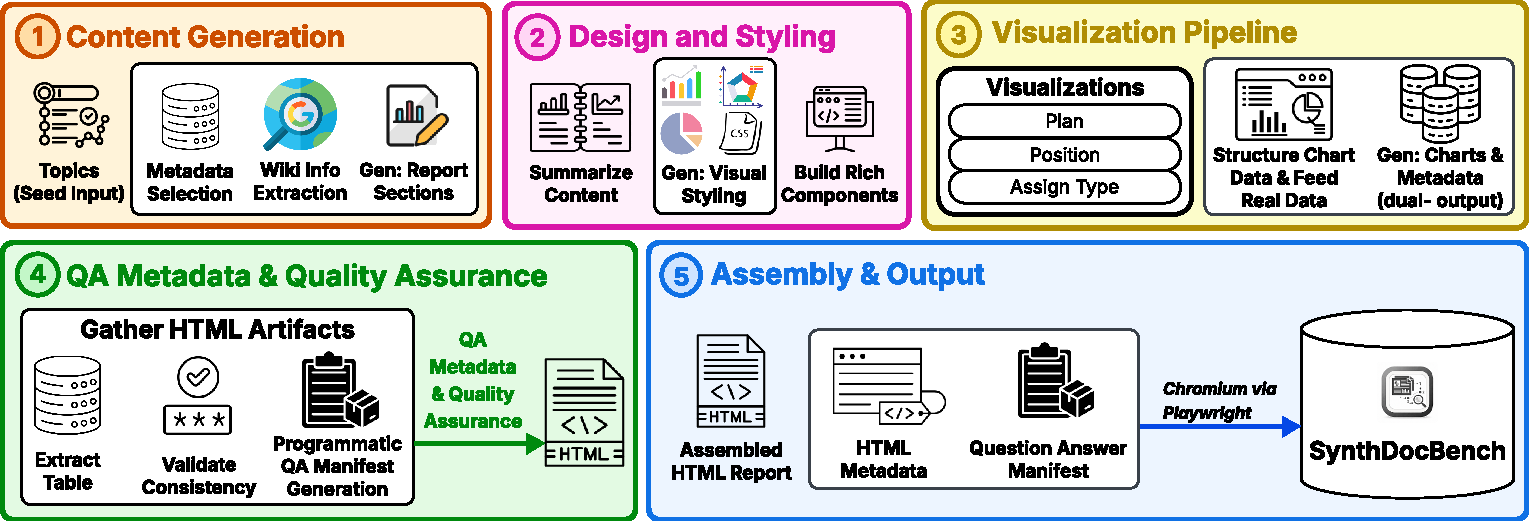
\includegraphics[width=\textwidth]{images/ReportGeneration.pdf}
  \vspace{4pt}
  \caption{
    \textbf{Synthetic visual document generation pipeline.}
   From a topic seed, the pipeline generates grounded report content, applies document-level visual styling, synthesizes visualizations, performs metadata and QA validation, and assembles the final HTML/PDF reports with a machine-readable QA manifest.
  }
  \label{fig:report_pipeline}
\end{figure}

\textbf{Topic-grounded content generation:} Given $\tau$, the pipeline constructs a semantic backbone from retrieved topic-relevant evidence and reorganizes it into a structured intermediate representation that exposes section boundaries, data-bearing spans, and salient content units. Downstream stages operate over this representation rather than free-form text, enabling precise evidence tracing. \\
\textbf{Design and visual grammar:} A layout archetype $a \in \mathcal{A}$ is sampled with probability 0.6 from a topic-conditioned distribution and with probability 0.4 uniformly at random (see Appendix~\ref{app:archetypes}), preventing trivial correlations between subject matter and layout. The archetype governs page grammar, chart placement strategy, and auxiliary component types (metric cards, timelines, pull quotes), yielding a realistic and diverse report distribution. \\
\textbf{Grounded visualization synthesis:} Each visualization is generated in two aligned forms: (i)~a visible D3.js rendering that appears in the document, and (ii)~a structured metadata object $V_k$ recording chart semantics (axes, data points, derived insights). This \emph{dual-layer} formulation ensures ground truth is available by construction without post-hoc chart parsing or human labeling (full schema in Appendix~\ref{app:viz_schema}). \\
\textbf{Validation and assembly:} Numeric values in both chart and table metadata are recomputed from structured data and corrected before finalization; all validated metadata are aggregated into $\mathcal{M}$. The report is assembled as HTML and rendered to PDF using Playwright,\footnote{\url{https://github.com/microsoft/playwright}} producing an aligned pair $(\mathcal{D}, \mathcal{M})$.

% ============================================================
\subsection{Question-Answer Generation}
\label{sec:pipeline:qa}
% ============================================================

The second stage converts a generated report into structured QA items via evidence recovery, synthesis, and generation with validation (Figure~\ref{fig:qa_pipeline}).

\begin{figure}[t]
  \centering
  \vspace{4pt}
  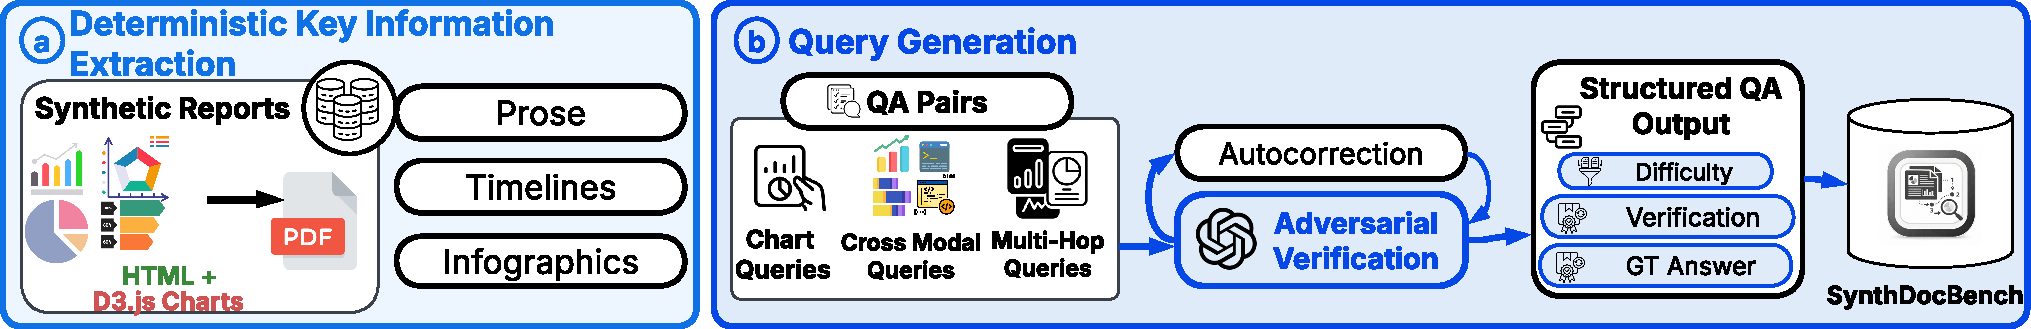
\includegraphics[width=\textwidth]{images/QnAGen.pdf}
  \vspace{4pt}
  \caption{%
    \textbf{QA generation pipeline.}
    The pipeline parses the generated report into structured evidence channels, extracts and synthesizes key information, and generates chart-reading, cross-modal, and multi-hop questions. A verification stage filters weak or malformed items before serializing the final QA output.%
  }
  \label{fig:qa_pipeline}
\end{figure}

The pipeline parses $\mathcal{D}$ into text, table, and visualization channels, recovering chart semantics directly from embedded metadata rather than pixels. Evidence units are then synthesized into higher-order compositions supporting aggregation, comparison, and cross-source reasoning.

The benchmark produces three question families: \emph{chart-reading} (direct chart or table semantics), \emph{cross-modal} (joint reasoning over textual and visual evidence), and \emph{complex multi-hop} (composition across 2--4 evidence units). Each question carries a difficulty label $L1$--$L5$ (Table~\ref{tab:difficulty-levels}) and a structured evidence trace. A validation stage filters malformed, weakly supported, or ambiguous items; the serialized output schema is detailed in Appendix~\ref{app:qa_schema}. Three-layer quality control (numeric recomputation, automated consistency filtering, and 100-sample manual review with $>$96\% acceptance rate) is described in Appendix~\ref{app:qc}.

\subsection{Benchmark Statistics}
\label{app:doc_stats}
% ──────────────────────────────────────────────────────────────


\begin{table}
  \centering
  \label{tab:doc_stats}
  \small
  \resizebox{0.42\textwidth}{!}{%
  \begin{tabular}{lrrrr}
    \toprule
    \textbf{Metric} & \textbf{Mean} & \textbf{Med.} & \textbf{Min} & \textbf{Max} \\
    \midrule
    Pages           & 51.1   & 49     & 24     & 91     \\
    Words           & 20,568 & 20,450 & 17,367 & 25,138 \\
    Charts          & 16.7   & 14     &  5     & 32     \\
    PDF (MB)        & 2.12   & 2.10   & 1.20   & 3.80   \\
    \bottomrule
  \end{tabular}%
  }
  \caption{Per-document statistics across all 200 reports.}
\end{table}


The resulting benchmark comprises \textbf{200 synthetic reports} and \textbf{1,788 questions}
distributed across three subsets: 597 \texttt{chart} reading,
597 \texttt{complex} multi-hop, and 594 \texttt{cross\_modal}.
Documents average \textbf{51.1 pages}, \textbf{16.7 charts}, and \textbf{$\approx$20,568 words},
placing \textsc{SynthDocBench} firmly in the long-document regime.
The benchmark spans \textbf{24 distinct chart types} across \textbf{6 layout archetypes},
ensuring models cannot exploit narrow visual or structural distributions.
Figure~\ref{fig:doc_composition} shows the distributions of page count, word count,
and chart count per document: all three are unimodal and tightly concentrated,
reflecting the controlled generation pipeline rather than the heavy-tailed distributions
typical of real-world corpora.
The tight ranges reflect the controlled generation pipeline: page count,
word count, and chart count are all bounded by design, enabling ablations
that hold document complexity constant while varying other axes (modality,
question type, layout).

\begin{figure}[htbp]
  \centering
  \begin{minipage}[t]{0.62\linewidth}
    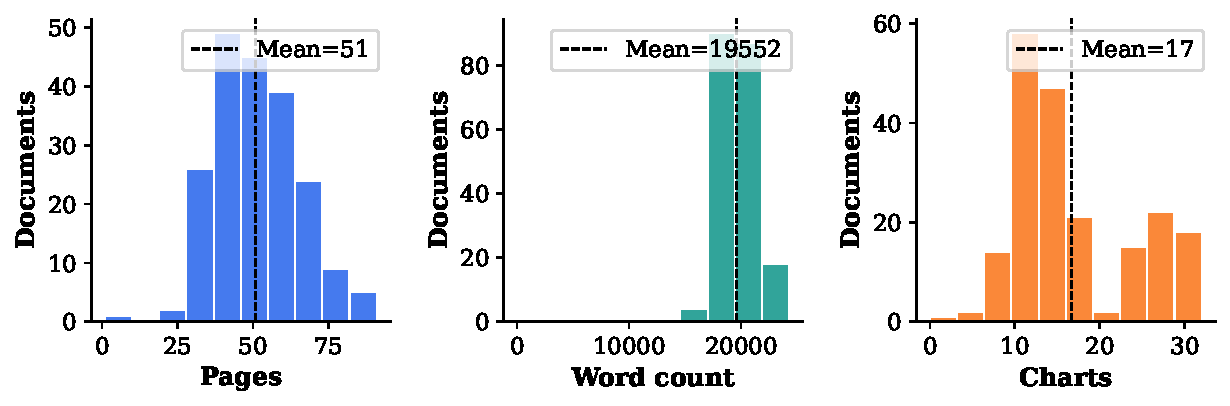
\includegraphics[width=\linewidth]{images/fig_doc_properties.pdf}
    \vspace{4pt}
    {\small\textit{(a) Document property distributions (pages, words, charts).}}
  \end{minipage}
  \hspace{0.04\linewidth}\hfill
  \begin{minipage}[t]{0.28\linewidth}
    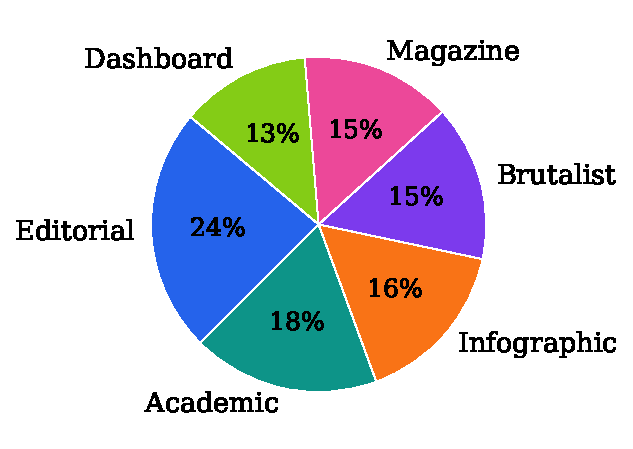
\includegraphics[width=\linewidth]{images/fig_archetype_dist.pdf}
    \vspace{4pt}
    {\small\textit{(b) Layout archetypes}}
  \end{minipage}
  \caption{Document composition statistics across 200 reports.}
  \label{fig:doc_composition}
\end{figure}

% \begin{figure}[t]
%   \centering
%   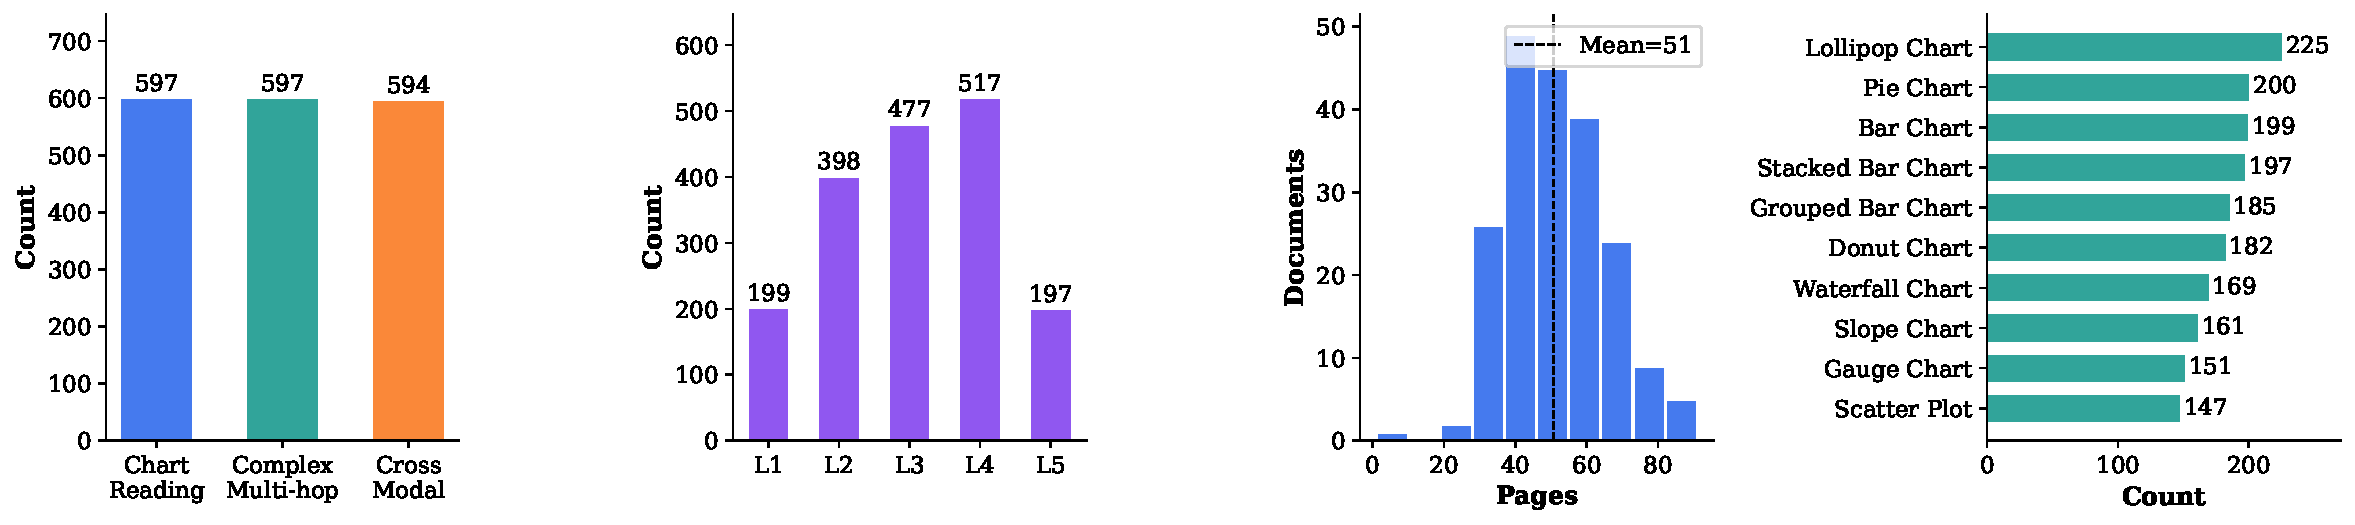
\includegraphics[width=\linewidth]{images/fig_dataset_overview.pdf}
%   \caption{Overview of \textsc{SynthDocBench} dataset statistics.
%     (a)~Questions are balanced equally across the three subsets.
%     (b)~Difficulty is skewed toward levels L3--L4 to stress compositional reasoning.
%     (c)~Documents span 38--65 pages (mean~50.8), covering realistic long-context conditions.
%     (d)~24 distinct chart types appear across the corpus, ensuring visual vocabulary diversity.}
%   \label{fig:dataset_overview}
% \end{figure}
